\documentclass[10pt, a4paper]{article}
\usepackage{ctex}
\usepackage{amsfonts}
\usepackage{amsmath}
\usepackage{amssymb, bm}
\usepackage{algorithm}
\usepackage{algpseudocode}
\usepackage{hyperref}
\usepackage[top=25.4mm, bottom=25.4mm, left=31.7mm, right=32.2mm]{geometry}
\usepackage{graphicx}
\usepackage{subfigure}
\usepackage{booktabs}
% \usepackage{float}
% \usepackage{subfig}


\setmainfont{Times New Roman}
\newtheorem{property}{性质}[section]
\newtheorem{thm}{定理}[section]
\newtheorem{definition}{定义}[section]
\renewcommand{\algorithmicrequire}{\textbf{输入:}}
\renewcommand{\algorithmicensure}{\textbf{输出:}}

\usepackage[
    style=numeric,
    sorting=none,
    bibstyle=gb7714-2015,
    citestyle=gb7714-2015
]{biblatex}

\renewcommand{\bibfont}{\zihao{-5}}

\addbibresource{reference.bib}

\begin{document}
\begin{titlepage}
\pagenumbering{Roman}
\author{张皓飞 (11921056)}
\title{语义分割模型:DeepLab}
\maketitle
\thispagestyle{empty}
\end{titlepage}

\newpage
\tableofcontents
\newpage
\pagenumbering{arabic}

\section{引言}
\subsection{计算机视觉中的任务}
计算机视觉想要解决的问题就是如何让机器真正理解一张输入图片,那么首先,机器必须要知道这张图片所描述的对象是什么。
比较简单的做法就是将所有图像描述的对象划分成一系列的类别,并对输入的图片根据划分好的类别进行分类,这样机器就可以
获得输入图片的最基本语义信息。因此分类问题就是计算机视觉中是一个至关重要的任务。

传统的解决分类的任务为先根据输入的图片的大致分布人为构建一系列特征提取器,比较有名的特征提取器为SIFT\cite{SIFT}、
SURF\cite{SURF}和HOG\cite{HOG}等。这些特征提取器将输入的图像变换为具有固定长度的向量,之后再使用线性分类器如
Rosenblatt感知机\cite{Rosenblatt}、贝叶斯分类器\cite{SimonNNLM}和支持向量机(SVM)\cite{SVM-Kernel}等
或非线性的分类器如决策树\cite{DataMining}、基于核方法的支持向量机\cite{SVM-Kernel}进行分类。

尽管这些传统的图像分类算法具有严格证明的数学定理和证明做支撑,但由于分类器以及研究得非常透彻,以至于大部分的算法
构建时间都会用在如何从图像提取特征的问题,也称为“特征工程”。由于图像的分布对于不同的任务差异巨大,以至于这些
特征工程算法很难进行泛化和推广,因此研究人员需要花费大量的时间进行模型的调参,从而得到令人满意的结果。

随着计算机软硬件和互联网的蓬勃发展,研究人员可以获得大量的数据,然而模型的效果并没有随着数据量的增加而显著提高,
而于此同时,基于卷积神经网络的分类器却显著地由于传统的特征工程方法。在2012年的ILSVRC\cite{ILSVRC}的比赛中
Alex Krizhevsky通过训练卷积神经网络AlexNet\cite{AlexNet}并获得了冠军。

尽管卷积神经网络并没有像传统机器学习一样具有很强的可解释性,但由于其可表述更强的非线性性和更大的参数空间,使得
深度模型可以往往收敛到较传统方法更优的模型。

\subsection{语义分割任务}
有了对图片的分类,机器可以初步理解图像所表示的类别,但是通常图片里具有多个物体,每个物体可能都属于不同的类别,
因此我们希望机器可以对一张图片的所有物体全部标记在图像中,从而可以获取到图片中更多的信息。从本质上将,
语义分割任务即对输入的图片的每个像素点进行分类,并将相同类别的像素点进行组合,从而得到物体对应的位置。

有了对图片的语义分割,我们可以获得更高层次的语义信息。在自动驾驶、人机交互和虚拟现实等诸多应用中都需要输入图片的
更高层次的语义信息。因此语义分割任务也是计算机视觉里重要的任务之一。

本文中将介绍一种基于深度卷积网络的语义分割模型DeepLab\cite{Deeplab1,Deeplab2,Deeplab3}系列,
该算法在Pascal VOC数据集\cite{VOC}和MSCOCO数据集\cite{COCO}取得了当时较好的结果。

\section{相关工作}
\subsection{语义分割任务}
关于深度卷积网络(DCNNs)在像素级语义分割中有大致三种主要方法:

\begin{description}
    \item[基于区域的语义分割] 基于区域的方法通常基于目标检测架构如R-CNN\cite{RCNN}等,对于分割的任务,R-CNN首先利用
    选择性搜索提取大量的候选区域,并计算其对应的特征。之后再使用线性分类模型对每个区域进行分类,再将区域的预测转换为
    像素预测。这种方法通常无法端到端实现,计算量较大。
    \item[弱监督语义分割] 通常对语义分割的数据集的标注是非常繁琐的,为此许多方法提出使用边框注释来作为监督信息训练
    模型,而非像素级的标注如BoxSup\cite{BoxSup}算法致力于通过使用带注释的边界框来实现语义分割。
    \item[全卷积网络语义分割] 全卷积网络可以对输入的图像进行端到端的语义分割,从而使得语义分割模型可以快速且方便的训练。
    全卷积网络大致可看成为编码器-解码器架构,其中编码器部分从图像中提取特征,解码器部分将提取到的特征恢复为语义分割的图像,
    如图\ref{p1}所示。目前,FCNs\cite{FCN}、SegNet\cite{SegNet}以及U-Net\cite{UNet}系列模型都为基于全卷积的
    语义分割模型类别中。

    \begin{figure}[htbp]
        \centering
        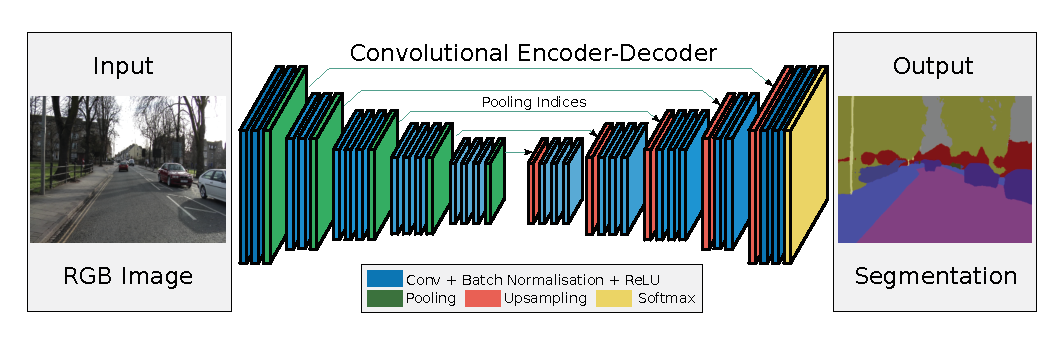
\includegraphics[width=\textwidth]{imgs/p1.eps}
        \caption{编解码器示例\cite{SegNet}}
        \label{p1}
    \end{figure}
\end{description}

尽管DeepLab系列模型并不完全可以划分到上面三类,但由于其整体依旧可看作编-解码器类型,因此本文中将DeepLab划分到
全卷积网络语义分割。为此我们需要简单介绍编解码器架构。

\subsection{编-解码器架构}
在编-解码的模型框架中,整体可以看作两部分:第一部分为编码器,负责将输入的图片转换为在编码子空间中对输入图像的表示
(嵌入);第二部分为解码器,负责将编码子空间中的表示恢复到维度更高的子空间中,如输入图像的子空间。在这种架构中,
编码器可以将图像里复杂的目标提取出来,并剔除部分噪声。解码器部分则试图按照任务要求构将编码的信息部分恢复。
在编-解码器的框架下,可以完成如语义分割,图像降噪,超分辨等任务。

一般而言,编码器部分为深度卷积神经网络,且采用最大池化等操作进行维度的缩减,这样可以使得网络具有缩放不变性,平移不变性等。
在解码器部分,通常采用转置卷积的操作以恢复维度。

\section{方法}
\subsection{DeepLab-V1}
在第一版的DeepLab模型中,使用DCNNs做为输入图像的特征提取器和稠密图像分类器,像素级的全连接条件随机场(CRFs)\cite{CRF}
作为语义分割部分。其编码器部分可以看作是稠密图像分类器,解码器部分可以看作为全连接条件随机场。

\subsubsection{稠密图像分类器}
DeepLab使用在ImageNet数据集预训练的VGG-16模型\cite{VGG}作为骨干网络。然而在分类任务中强调目标的平移不变性,
而在像素级语义分割中,则需要平移可变性。因此,DeepLab方法将VGG模型中的后两次池化层去掉,并使将最后三次卷积操作
变成空洞卷积如图\ref{p2}所示。从而将输入图像的尺寸降低到原来的$\frac{1}{8}$,并作为图像的表示。

和池化操作或者步长不为1的卷积操作相比,空洞卷积操作可以在降低维度的同时具有更大的感受野,这样就可以在保留更多的空间
信息的同时降低维度。尽管我们可以不设置池化操作,从而维持每层网络的输出不变,然而这样会导致计算量的增加,使得网络更加
难以优化。

\begin{figure}[htbp]
    \centering
    \includegraphics[width=7cm]{imgs/p2.png}
    \caption{一维空洞卷积示例,这里卷积核大小为3,输入的步长为2,输出的步长为1}
    \label{p2}
\end{figure}

\subsubsection{全连接条件随机场}
在稠密图像分类器中,在一定程度上我们可以得到语义分割的结果(尺度为原来的$\frac{1}{8}$),但由于深度卷积网络在准确率和
定位上的矛盾,因此直接使用DCNNs的输出结果效果不佳。为了解决该问题,研究人员提出了两个解决的方向,一是采用多层输出的信息来
对目标的边界进行更好的确定\cite{FCN,eigen2015predicting};另外一类方法采用超像素的表示,将定位变成一种低级的分割方法
\cite{mostajabi2015feedforward}。而在DeepLab算法中,给出了一种新的解决思路,即结合DCNNs的识别能力以及全连接条件
随机场的细粒度定位能力。

传统上,条件随机场是用来对分割结果进行光滑处理,通常这些模型包含耦合相邻节点的能量项,倾向于将相同的标签分配给空间上最接近的
像素。这些短程的条件随机场的主要功能为清楚奖励在手工设计的特征上的弱分类器的虚假预测。而从图\ref{p3}中我们可以看到,DCNNs
输出的结果已经非常光滑,因此我们的目的不是对其进行光滑处理,而是恢复细节信息。为此DeepLab引入全连接条件随机场的模型\cite{FC-CRF}
来进行更细致的语义分割。

\begin{figure}[htbp]
    \centering
    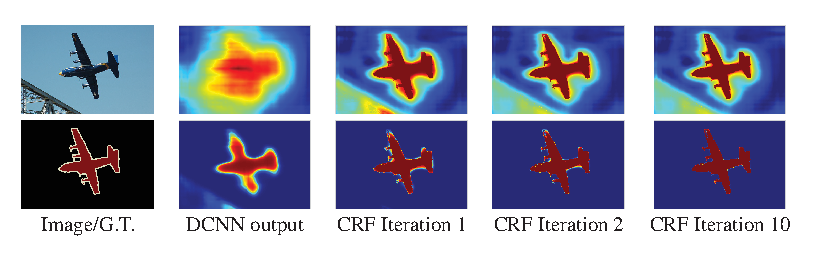
\includegraphics[width=\textwidth]{imgs/p3.eps}
    \caption{使用DCNN和全连接条件随机场做分割的比较,其中最左面的为真实标注结果}
    \label{p3}
\end{figure}

定义能量函数
\begin{equation}
    E(\bm{x}) = \sum_i \theta_i(x_i) + \sum_{i,j}\theta_{i, j}(x_i, x_j)
\end{equation}

其中$\bm{x}$为对每个像素的标签。使用一元势函数$\theta_i(x_i) = -\log P(x_i)$,其中函数$P(x_i)$为通过DCNN得到的
对像素$i$的概率标签。二元势函数定义为
\[
    \theta_{i, j}(x_i, x_j) = \mu(x_i, x_j)\sum_{m=1}^K w_m\cdot k^m(\bm{f}_i, \bm{f}_j)
\]
其中,
\[
    \mu(x_i, x_j) = 
    \begin{cases}
        1 & x_i \neq x_j \\
         0 & x_i = x_j
    \end{cases} 
\]

每一个函数$k_m(\cdot, \cdot)$,都为高斯个函数都依赖于第$i$和第$j$个像素点的特征。DeepLab采用双边位置和颜色项并进行加权
\begin{equation}
    w_1\exp\left(-\frac{\|p_i - p_j\|^2}{2\sigma_\alpha^2} - \frac{\|I_i - I_j\|^2}{2\sigma_\beta^2}\right) + 
    w_2\exp\left(-\frac{\|p_i - p_j\|^2}{2\sigma_\gamma^2}\right)
\end{equation}

其中第一项依赖于像素点$i$和$j$的距离和像素的值,而第二项仅依赖于距离,$\sigma_\alpha$、$\sigma_\beta$和$\sigma_\gamma$
均为高斯核函数的超参数。

\subsubsection{小结}
DeepLab第一个版本的整体流程如图\ref{p4}所示,首先输入的图片经过深度卷积网络得到粗粒度的分割图,经过双线新插值后
恢复原图的尺寸,再通过全连接条件随机场获得最终的语义分割结果。
\begin{figure}[htbp]
    \centering
    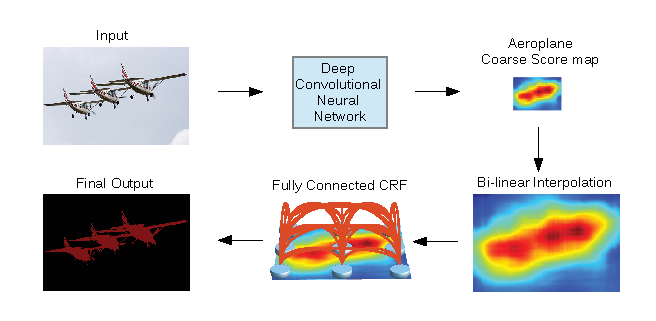
\includegraphics[width=\textwidth]{imgs/p4.eps}
    \caption{模型整体流程}
    \label{p4}
\end{figure}

\subsection{DeepLab-V2}
DeepLab-V2为对上述DeepLab-V1模型的改进,主要改进为将原模型中DCNN中的空洞卷积进行改进,采用多个上采样的卷积核组合构成
多孔卷积(Atrous Convolution),此外在DeepLab-V2中骨架网络由原来的VGG改为ResNet-101\cite{ResNet}。

\subsubsection{多孔卷积}
在模型DeepLab-V1中,采用空洞卷积来避免对输入图片的空间信息的丢失。在本模型中,目标依然是进一步增加空间信息。
为此,采用多个不同孔径大小的空洞卷积核组成多孔空间金字塔池化层(ASPP)如图\ref{p5}所示,其本质为多尺度的
空洞卷积的叠加其具体实现如图\ref{p6}所示。
\begin{figure}[h]
    \centering
    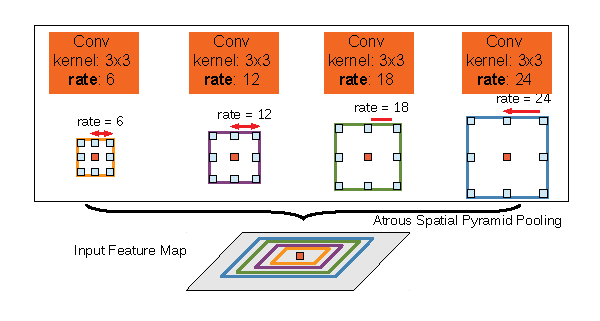
\includegraphics[width=10cm]{imgs/p5.eps}
    \caption{ASPP示例}
    \label{p5}
\end{figure}

\begin{figure}[h]
    \centering
    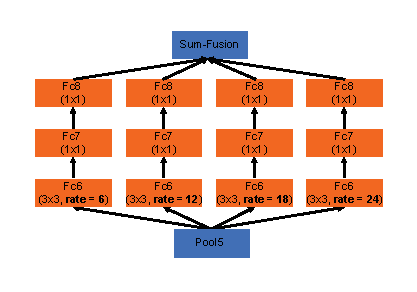
\includegraphics[width=10cm]{imgs/p6.eps}
    \caption{ASPP实现方式}
    \label{p6}
\end{figure}

\subsection{DeepLab-V3}
在DeepLab-V3模型中,同样使用ResNet作为骨架网络如图\ref{p7}所示,网络前3个块直接使用了ResNet的前3个块,其中每个
块里卷积层保持输入的维度,最后一层通过步长为2的卷积降低特征的维度。若直接使用ResNet的结构如\ref{p7-1},会导致最终输出的特征维度
过低,从而语义分割的位置精度下降。

而采用空洞卷积来加深网络如\ref{p7-2},可以在维持特征维度的情况下获取到更大的感受野,从而提高精度。最终,DeepLab-V3的改进如图\ref{p8}
所示。

\begin{figure}[htbp]
    \centering
    \subfigure[不使用空洞卷积加深网络]{
        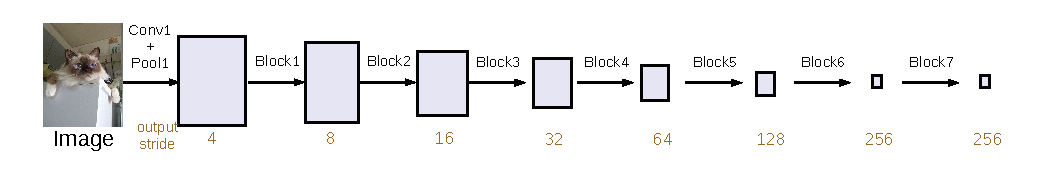
\includegraphics[width=\textwidth]{imgs/p7-1.eps}
        \label{p7-1}
    }
    \subfigure[使用空洞卷积加深网络]{
        \includegraphics[width=\textwidth]{imgs/p7-2.eps}
        \label{p7-2}
    }
    \caption{DCNNs加深方式示意}
    \label{p7}
\end{figure}

\begin{figure}[htbp]
    \centering
    \includegraphics[width=\textwidth]{imgs/p8.eps}
    \caption{改进ASPP实现方式}
    \label{p8}
\end{figure}

\section{实验结果}
本章中,我们将展示对模型DeepLab-V3复现的结果。复现环境如表\ref{t0}所示。

\begin{table}[htbp]
\begin{center}  
\begin{tabular}{ll}
    \toprule
    操作系统 & Ubuntu 18.04.4 LTS\\
    CPU & 双路 Intel \circledR Xeon \circledR Gold 5122 CPU @ 3.60GHz \\
    GPU & NVIDIA \circledR Quadro \circledR P6000 \\
    代码语言 & Python 3.7.4 \\
    深度学习框架 & PyTorch-1.5\\
    \bottomrule
\end{tabular}
\end{center}
\caption{复现环境}
\label{t0}
\end{table}

\subsection{数据集}
我们使用的数据集为Pascal VOC和Cityscapes数据集。
\begin{description}
    \item[Pascal VOC] 具体而言,我们使用Pascal VOC 2012分割数据集,分别包含1464,1449和1456张训练、验证和测试的图片。
    包括背景。主要包含真实场景中的物体,共计20个类别。
    \item[Cityscape] Cityscapes拥有5000张在城市环境中驾驶场景的图像,由19个类别的语义分割标注。
\end{description}

\subsection{其它设定}
模型的骨架网络使用了ResNet-50和ResNet-101。学习率按照表\ref{t1}设定。训练的循环次数按表\ref{t2}确定。

\begin{table}[!htbp]
\begin{center}  
\begin{tabular}{ll}
    \toprule
    数据集 & 学习率\\
    \midrule
    Pascal Voc & $0.0001$ \\
    Cityscapes & $0.01$ \\
    \bottomrule
\end{tabular}
\end{center}
\caption{学习率设定}
\label{t1}
\end{table}

\begin{table}[!htbp]
\begin{center}  
\begin{tabular}{ll}
    \toprule
    数据集 & 循环次数\\
    \midrule
    Pascal Voc & $50$ \\
    Cityscapes & $120$ \\
    \bottomrule
\end{tabular}
\end{center}
\caption{训练循环次数}
\label{t2}
\end{table}

\subsection{训练结果}
DeepLab-V3的训练结果由表\ref{t3}给出。

\begin{table}[!htbp]
\begin{center}  
\begin{tabular}{llll}
        \toprule
        数据集 & 骨干模型 & 像素级准确率 & mIoU \\
        \midrule
        Pascal Voc & ResNet-50 & $84.618$ & $56.120$ \\
        Pascal Voc & ResNet-101 & $89.467$ & $66.315$ \\
        Cityscapes & ResNet-50 & $91.406$ & $57.478$ \\
        Cityscapes & ResNet-101 & $92.725$ & $62.548$ \\
        \bottomrule
\end{tabular}
\end{center}
\caption{DeepLab-V3模型在各数据集和骨干网络上的结果}
\label{t3}
\end{table}

在随机抽取的测试图片的分割结果如图\ref{p9},\ref{p10}所示,可以看出使用ResNet-101作为网络骨架训练出的结果要比
ResNet-50分割效果更好。


\begin{figure}[h]
    \centering
    \begin{minipage}[b]{0.8\linewidth}
    \subfigure[输入图像]{
    \begin{minipage}[b]{0.31\linewidth}
        \centering
        \includegraphics[width=\linewidth]{imgs/raw-2009_003044.jpg}\vspace{0pt}
        \includegraphics[width=\linewidth]{imgs/raw-2009_003375.jpg}\vspace{0pt}
        \includegraphics[width=\linewidth]{imgs/raw-2009_003399.jpg}\vspace{0pt}
        \includegraphics[width=\linewidth]{imgs/raw-2009_004375.jpg}
      \end{minipage}
    }
    % \hfill
    \subfigure[骨干网络为ResNet50]{
    \begin{minipage}[b]{0.31\linewidth}
        \centering
        \includegraphics[width=\linewidth]{imgs/r50-2009_003044.png}\vspace{0pt}
        \includegraphics[width=\linewidth]{imgs/r50-2009_003375.png}\vspace{0pt}
        \includegraphics[width=\linewidth]{imgs/r50-2009_003399.png}\vspace{0pt}
        \includegraphics[width=\linewidth]{imgs/r50-2009_004375.png}
      \end{minipage}
    }
    % \hfill
    \subfigure[骨干网络为ResNet101]{
    \begin{minipage}[b]{0.31\linewidth}
        \centering
        \includegraphics[width=\linewidth]{imgs/r101-2009_003044.png}\vspace{0pt}
        \includegraphics[width=\linewidth]{imgs/r101-2009_003375.png}\vspace{0pt}
        \includegraphics[width=\linewidth]{imgs/r101-2009_003399.png}\vspace{0pt}
        \includegraphics[width=\linewidth]{imgs/r101-2009_004375.png}
      \end{minipage}
    }
    \end{minipage}
    \vfill
    \caption{DeepLab不同的骨架网络在Pascal Voc数据集上用随机输入图片测试的结果}
    \label{p9}
\end{figure}

\begin{figure}[h]
    \centering
    \begin{minipage}[b]{0.8\linewidth}
    \subfigure[输入图像]{
    \begin{minipage}[b]{0.31\linewidth}
        \centering
        \includegraphics[width=\linewidth]{imgs/raw-berlin_000006_000019_leftImg8bit.png}\vspace{0pt}
        \includegraphics[width=\linewidth]{imgs/raw-bonn_000015_000019_leftImg8bit.png}\vspace{0pt}
        \includegraphics[width=\linewidth]{imgs/raw-leverkusen_000013_000019_leftImg8bit.png}\vspace{0pt}
        \includegraphics[width=\linewidth]{imgs/raw-munich_000079_000019_leftImg8bit.png}
      \end{minipage}
    }
    % \hfill
    \subfigure[骨干网络为ResNet50]{
    \begin{minipage}[b]{0.31\linewidth}
        \centering
        \includegraphics[width=\linewidth]{imgs/r50-berlin_000006_000019_leftImg8bit.png}\vspace{0pt}
        \includegraphics[width=\linewidth]{imgs/r50-bonn_000015_000019_leftImg8bit.png}\vspace{0pt}
        \includegraphics[width=\linewidth]{imgs/r50-leverkusen_000013_000019_leftImg8bit.png}\vspace{0pt}
        \includegraphics[width=\linewidth]{imgs/r50-munich_000079_000019_leftImg8bit.png}
      \end{minipage}
    }
    % \hfill
    \subfigure[骨干网络为ResNet101]{
    \begin{minipage}[b]{0.31\linewidth}
        \centering
        \includegraphics[width=\linewidth]{imgs/r101-berlin_000006_000019_leftImg8bit.png}\vspace{0pt}
        \includegraphics[width=\linewidth]{imgs/r101-bonn_000015_000019_leftImg8bit.png}\vspace{0pt}
        \includegraphics[width=\linewidth]{imgs/r101-leverkusen_000013_000019_leftImg8bit.png}\vspace{0pt}
        \includegraphics[width=\linewidth]{imgs/r101-munich_000079_000019_leftImg8bit.png}
      \end{minipage}
    }
    \end{minipage}
    \vfill
    \caption{DeepLab不同的骨架网络在Cityscapes数据集上用随机输入图片测试的结果}
    \label{p10}
\end{figure}

\section{总结}
DeepLab系列模型与常规的编-解码器框架不同点在于其采用了空洞卷积或组合的空洞卷积,并减少对池化或步长不为1的卷积的
应用,使得完了能够获得足够的感受野的情况下依然可以减少特征的尺寸,从而利用了深度卷积网络的分类准确率高的特性。
此外,通过应用全连接条件随机场,将卷积网络输出的稠密分类图进行尺寸扩张和锐化边缘,使得输出的语义分割图像可以具有
一方面像素分类的准确率高,另一方面对于物体的定位更加准确。

\clearpage
\newpage
\addcontentsline{toc}{section}{参考文献}
\nocite{*}
\printbibliography[heading=bibliography,title=参考文献]

\end{document}
